\documentclass[11pt]{article} 

% ------- List of packages to import ------------
\usepackage{fullpage}
\usepackage{soul}
\usepackage{url}
\usepackage{pgf}
\usepackage{tikz}
\usetikzlibrary{arrows,automata,positioning}
\usepackage[latin1]{inputenc}
\usepackage{clrscode3e} % Documentation here http://www.cs.dartmouth.edu/~thc/clrscode/clrscode3e.pdf
\usepackage{amssymb}
\usepackage{amsmath}
\RequirePackage[amsmath,hyperref,thmmarks]{ntheorem}
\usepackage{hyperref} % This always has to be the LAST package.  

\theoremseparator{.}

% ------- Theorem and related environments --------
\newtheorem{theorem}{Theorem}
\newtheorem{conjecture}[theorem]{Conjecture}
\newtheorem{proposition}[theorem]{Proposition}
\newtheorem{claim}[theorem]{Claim}
\newtheorem{lemma}[theorem]{Lemma}
\newtheorem{corollary}[theorem]{Corollary}
\newtheorem{definition}[theorem]{Definition} 
\newtheorem{problem}[theorem]{Problem}
\newtheorem{observation}[theorem]{Observation}
\newtheorem{fact}[theorem]{Fact}

% ------- Commands specifying theorem style -------

\theoremstyle{nonumberplain}
\theoremheaderfont{\normalfont\itshape}
\theorembodyfont{\normalfont}
\theoremsymbol{\ensuremath{_\blacksquare}}
\newtheorem{proof}{Proof}

% ------- Useful math macros -----------
\newcommand{\NN}{\mathcal{N}} % Natural Numbers
\newcommand{\RR}{\mathcal{R}} % Real Numbers
\newcommand{\ZZ}{\mathcal{Z}} % Integers
\newcommand{\QQ}{\mathcal{Q}} % Rational Numbers

\newcommand{\set}[1]{\ensuremath{\{{#1}\}}} % Set
\newcommand{\bigset}[1]{\ensuremath{\left\{{#1}\right\}}}
\newcommand{\condset}[2]{\ensuremath{\set{{#1}\;|\;{#2}}}} % Conditional set
\newcommand{\nin}{\not\in}
\newcommand{\cross}{\times} % Cartesian product
\newcommand{\ssn}{\subsetneq} % Proper subset
\newcommand{\sse}{\subseteq} % Subset

%% ^^^^^^^^^ Don't change anything above this line ^^^^^^^^^^^^^^^^


\title{Depth First Search and its Application in Topological Sort}  % Change me!
\author{Benjamin May}  % Change me!
\date{\today}

\begin{document}

\maketitle

\begin{abstract}
  A brief description of your report.
\end{abstract}


\section{A Section} % \section* would create section without section
                       % number.

You should organized your report into appropriate sections and
subsections (see Subsection~\ref{subsec:1}).  You may cite CLRS
heavily in your report \cite{CLRS09}.

\section{Another Section}

You can even directly cite theorems.

\begin{theorem}[{{\cite[Thm 8.1]{CLRS09}}}]  % Note: the extra {}'s are required.
  Any comparison sort algorithm requires $\Omega(n \log n)$
  comparisons in the worst case.
\end{theorem}

\subsection{A subsection}
\label{subsec:1}

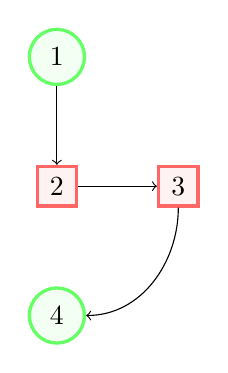
\begin{tikzpicture}[
roundnode/.style={circle, draw=green!60, fill=green!5, very thick, minimum size=7mm},
squarednode/.style={rectangle, draw=red!60, fill=red!5, very thick, minimum size=5mm},
]
%Nodes
\node[squarednode]      (maintopic)                              {2};
\node[roundnode]        (uppercircle)       [above=of maintopic] {1};
\node[squarednode]      (rightsquare)       [right=of maintopic] {3};
\node[roundnode]        (lowercircle)       [below=of maintopic] {4};

%Lines
\draw[->] (uppercircle.south) -- (maintopic.north);
\draw[->] (maintopic.east) -- (rightsquare.west);
\draw[->] (rightsquare.south) .. controls +(down:7mm) and +(right:7mm) .. (lowercircle.east);
\end{tikzpicture}

Look! we can make subsections.  We can also include figures and
images---see Figure~\ref{fig:bats}.

\begin{figure}[t] % Always use [t] for figures, never [h].
  \includegraphics[width=\linewidth]{bats.jpg}
  \caption{An example of a figure and how not to do this report.}
  \label{fig:bats} % Used to reference this figure in the text, it
                   % also worked with equations and algorithms.
\end{figure}

\subsubsection{A subsubsection}

and sub sub sections!

\paragraph{There are no subsubsubsections}

You may use a paragraph construct instead.

\section{Yet Another Section}

Put all your bibliographic entries in \texttt{report\_template.bib}.
If you locate the bibtex version of the citation you can just copy
that into the file.  Latex will automatically generate the citation
formating within your text and create a bibliography of the works
cited.  Lots more info about Latex bibliographies can be found at
\url{https://en.wikibooks.org/wiki/LaTeX/Bibliography_Management}.

\bibliographystyle{plain}
\bibliography{report_template} % This is referring to report_template.bib.

\end{document}
